% defer/rcuAPI.tex
% mainfile: ../perfbook.tex
% SPDX-License-Identifier: CC-BY-SA-3.0

\subsection{RCU Linux-Kernel API}
\label{sec:defer:RCU Linux-Kernel API}
\OriginallyPublished{Section}{sec:defer:RCU Linux-Kernel API}{RCU Linux-Kernel API}{Linux Weekly News}{PaulEMcKenney2008WhatIsRCUAPI}

This section looks at RCU from the viewpoint of its Linux-kernel API.\footnote{
	Userspace RCU's API is documented
	elsewhere~\cite{PaulMcKenney2013LWNURCU}.}
Section~\ref{sec:defer:RCU has a Family of Wait-to-Finish APIs}
presents RCU's wait-to-finish APIs,
Section~\ref{sec:defer:RCU has Publish-Subscribe and Version-Maintenance APIs}
presents RCU's publish-subscribe and version-maintenance APIs,
Section~\ref{sec:defer:RCU has List-Processing APIs}
presents RCU's list-processing APIs,
Section~\ref{sec:defer:RCU Has Diagnostic APIs}
presents RCU's diagnostic APIs, and
Section~\ref{sec:defer:Where Can RCU's APIs Be Used?}
describes in which contexts RCU's various APIs may be used.
Finally,
Section~\ref{sec:defer:So, What is RCU Really?}
presents concluding remarks.

Readers who are not excited about kernel internals may wish to skip
ahead to \cref{sec:defer:RCU Usage}
on page~\pageref{sec:defer:RCU Usage}.

\subsubsection{RCU has a Family of Wait-to-Finish APIs}
\label{sec:defer:RCU has a Family of Wait-to-Finish APIs}

The most straightforward answer to ``what is RCU'' is that RCU is
an API.
For example, the RCU implementation used in the Linux kernel is
summarized by
Table~\ref{tab:defer:RCU Wait-to-Finish APIs},
which shows the wait-for-readers portions of the RCU, ``sleepable'' RCU
(SRCU), Tasks RCU, and generic APIs, respectively,
and by
Table~\ref{tab:defer:RCU Publish-Subscribe and Version Maintenance APIs},
which shows the publish-subscribe portions of the
API~\cite{PaulEMcKenney2019RCUAPI}.\footnote{
	This citation covers v4.20 and later.
	Documetation for earlier versions of the Linux-kernel RCU API may
	be found elsewhere~\cite{PaulEMcKenney2008WhatIsRCUAPI,PaulEMcKenney2014RCUAPI}.}

\begin{sidewaystable*}[tbp]
\rowcolors{1}{}{lightgray}
\renewcommand*{\arraystretch}{1.3}
\centering
\caption{RCU Wait-to-Finish APIs}
\label{tab:defer:RCU Wait-to-Finish APIs}
\scriptsize\hspace*{-.125in}
\begin{tabularx}{8.5in}{>{\raggedright\arraybackslash}p{0.94in}
    >{\raggedright\arraybackslash}X
    >{\raggedright\arraybackslash}X
    >{\raggedright\arraybackslash}p{1.1in}
    >{\raggedright\arraybackslash}p{1.35in}
    >{\raggedright\arraybackslash}p{1.45in}}
\toprule
&
    {\bf RCU}: Original &
	{\bf SRCU}: Sleeping readers &
	    {\bf Tasks RCU}: Free tracing trampolines &
		{\bf Tasks RCU Rude}: Free idle-task tracing trampolines &
		    {\bf Tasks RCU Trace}: Protect sleepable BPF programs \\
\midrule
{\bf Read-side critical-section markers} &
    \tco{rcu_read_lock()}~! \tco{rcu_read_unlock()}~!
    \tco{rcu_read_lock_bh()} \tco{rcu_read_unlock_bh()}
    \tco{rcu_read_lock_sched()} \tco{rcu_read_unlock_sched()}
    (Plus anything disabing bottom halves, preemption, or interrupts.) &
	\tco{srcu_read_lock()} \tco{srcu_read_unlock()} &
	    Voluntary context switch &
		Voluntary context switch and preempt-enable regions of code &
		    \tco{rcu_read_lock_trace()} \tco{rcu_read_unlock_trace()} \\
{\bf Update-side primitives (synchronous) } &
    { \tco{synchronize_rcu()}
      \tco{synchronize_net()}
      \tco{synchronize_rcu_expedited()} } &
	\tco{synchronize_srcu()} \tco{synchronize_srcu_expedited()} &
	    \tco{synchronize_rcu_tasks()} &
		\tco{synchronize_rcu_tasks_rude()} &
		    \tco{synchronize_rcu_tasks_trace()} \\
{\bf Update-side primitives (asynchronous / callback) } &
    \tco{call_rcu()} ! &
	\tco{call_srcu()} &
	    \tco{call_rcu_tasks()} &
		\tco{call_rcu_tasks_rude()} &
		    \tco{call_rcu_tasks_trace()} \\
{\bf Update-side primitives (wait for callbacks) } &
    \tco{rcu_barrier()} &
	\tco{srcu_barrier()} &
	    \tco{rcu_barrier_tasks()} &
		\tco{rcu_barrier_tasks_rude()} &
		    \tco{rcu_barrier_tasks_trace()} \\
{\bf Update-side primitives (initiate / wait)} &
    \tco{get_state_synchronize_rcu()}
    \tco{cond_synchronize_rcu()} &
	&
	    &
		&
		    \\
{\bf Update-side primitives (free memory) } &
    \tco{kfree_rcu()} &
	&
	    &
		&
		    \\
{\bf Type-safe memory } &
    \tco{SLAB_TYPESAFE_BY_RCU} &
	&
	    &
		&
		    \\
{\bf Read side constraints } &
    No blocking (only preemption) &
	No \tco{synchronize_srcu()} with same \tco{srcu_struct} &
	    No voluntary context switch &
		Neither blocking nor preemption &
			No RCU tasks trace grace period \\
{\bf Read side overhead } &
    CPU-local accesses (\tco{barrier()} on \tco{PREEMPT=n}) &
	Simple instructions, memory barriers &
	    Free &
		CPU-local accesses (free on \tco{PREEMPT=n}) &
		    CPU-local accesses \\
{\bf Asynchronous update-side overhead } &
    sub-microsecond &
	sub-microsecond &
	    sub-microsecond &
		sub-microsecond &
		    sub-microsecond \\
{\bf Grace-period latency } &
    10s of milliseconds &
        Milliseconds &
	    Seconds &
		Milliseconds &
		    10s of milliseconds \\
{\bf Expedited grace-period latency } &
    10s of microseconds &
        Microseconds &
	    N/A &
		N/A &
		    N/A \\
\bottomrule
\end{tabularx}
\end{sidewaystable*}

If you are new to RCU, you might consider focusing on just one
of the columns in
Table~\ref{tab:defer:RCU Wait-to-Finish APIs},
each of which summarizes one member of the Linux kernel's RCU API family.
For example, if you are primarily interested in understanding how RCU
is used in the Linux kernel, ``RCU'' would be the place to start,
as it is used most frequently.
On the other hand, if you want to understand RCU for its own sake,
``Task RCU'' has the simplest API.
You can always come back for the other columns later.

If you are already familiar with RCU, these tables can
serve as a useful reference.

\QuickQuiz{
	Why do some of the cells in
	Table~\ref{tab:defer:RCU Wait-to-Finish APIs}
	have exclamation marks (``!'')?
}\QuickQuizAnswer{
	The API members with exclamation marks (\co{rcu_read_lock()},
	\co{rcu_read_unlock()}, and \co{call_rcu()}) were the
	only members of the Linux RCU API that Paul E. McKenney was aware
	of back in the mid-90s.
	During this timeframe, he was under the mistaken impression that
	he knew all that there is to know about RCU.
}\QuickQuizEnd

The ``RCU'' column corresponds to the consolidation of the
three Linux-kernel RCU
implementations~\cite{PaulEMcKenney2019RCUCVE,McKenney:2019:CRS:3319647.3325836},
in which RCU read-side critical sections start with
\co{rcu_read_lock()}, \co{rcu_read_lock_bh()}, or \co{rcu_read_lock_sched()}
and end with \co{rcu_read_unlock()}, \co{rcu_read_unlock_bh()},
or \co{rcu_read_unlock_sched()}, respectively.
Any region of code that disables bottom halves, interrupts, or preemption
also acts as an RCU read-side critical section.
RCU read-side critical sections may be nested.
The corresponding synchronous update-side primitives,
\co{synchronize_rcu()} and \co{synchronize_rcu_expedited()}, along with
their synonym \co{synchronize_net()}, wait for any type of currently
executing RCU read-side critical sections to complete.
The length of this wait is known as a ``grace period'', and
\co{synchronize_rcu_expedited()} is designed to reduce grace-period
latency at the expense of increased CPU overhead and IPIs.
The asynchronous update-side primitive, \co{call_rcu()},
invokes a specified function with a specified argument after a
subsequent grace period.
For example, \co{call_rcu(p,f);} will result in
the ``RCU callback'' \co{f(p)}
being invoked after a subsequent grace period.
There are situations,
such as when unloading a Linux-kernel module that uses \co{call_rcu()},
when it is necessary to wait for all
outstanding RCU callbacks to complete~\cite{PaulEMcKenney2007rcubarrier}.
The \co{rcu_barrier()} primitive does this job.

\QuickQuizSeries{%
\QuickQuizB{
	How do you prevent a huge number of RCU read-side critical
	sections from indefinitely blocking a \co{synchronize_rcu()}
	invocation?
}\QuickQuizAnswerB{
	There is no need to do anything to prevent RCU read-side
	critical sections from indefinitely blocking a
	\co{synchronize_rcu()} invocation, because the
	\co{synchronize_rcu()} invocation need wait only for
	\emph{pre-existing} RCU read-side critical sections.
	So as long as each RCU read-side critical section is
	of finite duration, RCU grace periods will also remain
	finite.
}\QuickQuizEndB
%
\QuickQuizE{
	The \co{synchronize_rcu()} API waits for all pre-existing
	interrupt handlers to complete, right?
}\QuickQuizAnswerE{
	In v4.20 and later Linux kernels,
	yes~\cite{PaulEMcKenney2019RCUCVE,McKenney:2019:CRS:3319647.3325836}.

	But not in earlier kernels, and especially not when using
	preemptible RCU!
	You instead want \co{synchronize_irq()}.
	Alternatively, you can place calls to \co{rcu_read_lock()}
	and \co{rcu_read_unlock()} in the specific interrupt handlers that
	you want \co{synchronize_rcu()} to wait for.
	But even then, be careful, as preemptible RCU will not be guaranteed
	to wait for that portion of the interrupt handler preceding the
	\co{rcu_read_lock()} or following the \co{rcu_read_unlock()}.
}\QuickQuizEndE
}

Finally, RCU may be used to provide
type-safe memory~\cite{Cheriton96a}, as described in
Section~\ref{sec:defer:RCU Provides Type-Safe Memory}.
In the context of RCU, type-safe memory guarantees that a given
data element will not change type during any RCU read-side critical section
that accesses it.
To make use of RCU-based type-safe memory, pass
\co{SLAB_TYPESAFE_BY_RCU} to \co{kmem_cache_create()}.

The ``SRCU'' column in
Table~\ref{tab:defer:RCU Wait-to-Finish APIs}
displays a specialized RCU API that permits general sleeping in SRCU
read-side critical
sections~\cite{PaulEMcKenney2006c}
delimited by \co{srcu_read_lock()} and \co{srcu_read_unlock()}.
However, unlike RCU, SRCU's \co{srcu_read_lock()} returns a value that
must be passed into the corresponding \co{srcu_read_unlock()}.
This difference is due to the fact that the SRCU user allocates an
\co{srcu_struct} for each distinct SRCU usage.
These distinct \co{srcu_struct} structures prevent SRCU read-side critical
sections from blocking unrelated \co{synchronize_srcu()} and
\co{synchronize_srcu_expedited()} invocations.
Of course, use of either \co{synchronize_srcu()} or
\co{synchronize_srcu_expedited()} within an SRCU read-side critical
section can result in self-deadlock, so should be avoided.
As with RCU, SRCU's \co{synchronize_srcu_expedited()} decreases
grace-period latency compared to \co{synchronize_srcu()}, but at
the expense of increased CPU overhead.

\QuickQuiz{
	Under what conditions can \co{synchronize_srcu()} be safely
	used within an SRCU read-side critical section?
}\QuickQuizAnswer{
	In principle, you can use either \co{synchronize_srcu()} or
	\co{synchronize_srcu_expedited()} with a given \co{srcu_struct}
	within an SRCU read-side critical section that uses some other
	\co{srcu_struct}.
	In practice, however, doing this is almost certainly a bad idea.
	In particular, the code shown in
	Listing~\ref{lst:defer:Multistage SRCU Deadlocks}
	could still result in deadlock.

\begin{listing}[htbp]
\begin{VerbatimL}
idx = srcu_read_lock(&ssa);
synchronize_srcu(&ssb);
srcu_read_unlock(&ssa, idx);

/* . . . */

idx = srcu_read_lock(&ssb);
synchronize_srcu(&ssa);
srcu_read_unlock(&ssb, idx);
\end{VerbatimL}
\caption{Multistage SRCU Deadlocks}
\label{lst:defer:Multistage SRCU Deadlocks}
\end{listing}
}\QuickQuizEnd

Similar to normal RCU, self-deadlock can be avoided using the
asynchronous \co{call_srcu()} function.
However, special care must be taken when using \co{call_srcu()} because
a single task could register SRCU callbacks very quickly.
Given that SRCU allows readers to block for arbitrary periods of
time, this could consume an arbitrarily large quantity of memory.
In contrast, given the synchronous \co{synchronize_srcu()}
interface, a given task must finish waiting for a given grace period
before it can start waiting for the next one.

Also similar to RCU, there is an \co{srcu_barrier()} function that waits
for all prior \co{call_srcu()} callbacks to be invoked.

In other words, SRCU compensates for its extremely weak
forward-progress guarantees by permitting the developer to restrict
its scope.

The ``Tasks RCU'' column in
\cref{tab:defer:RCU Wait-to-Finish APIs} displays a specialized
RCU API that mediates freeing of the trampolines used in Linux-kernel
tracing.
These trampolines are used to transfer control from a point in the
code being traced to the code doing the actual tracing.
It is of course necessary to ensure that all code executing within
a given trampoline has finished before freeing that trampoline.

Changes to the code being traced are typically limited to a single jump
or call instruction, and thus cannot accommodate the sequence of code
required to implement \co{rcu_read_lock()} and \co{rcu_read_unlock()}.
Nor can the trampoline contain calls to \co{rcu_read_lock()} and
\co{rcu_read_unlock()}.
To see this, consider a CPU that is just about to start executing a
given trampoline.
Because it has not yet executed the \co{rcu_read_lock()}, that
trampoline could be freed at any time, which would come as a fatal
surprise to this CPU.
Therefore, trampolines cannot be protected by synchronization primitives
executed in either the traced code or in the trampoline itself.
Which does raise the question of exactly how the trampoline is to be
protected.

The key to answering this question is to note that trampoline code
never contains code that either directly or indirectly does a
voluntary context switch.
This code might be preempted, but it will never directly or indirectly
invoke \co{schedule()}.
This suggests a variant of RCU having voluntary context switches and
idle execution as its only quiescent states.
This variant is Tasks RCU.

Tasks RCU is unusual in having no read-side marking functions, which
is good given that its main use case has nowhere to put such markings.
Instead, calls to \co{schedule()} serve directly as quiescent states.
Updates can use \co{synchronize_rcu_tasks()} to wait for all pre-existing
trampoline execution to complete, or they can use its asynchronous
counterpart, \co{call_rcu_tasks()}.
There is also an \co{rcu_barrier_tasks()} that waits for completion
of callbacks corresponding to all prior invocations of \co{call_rcu_tasks()}.
There is no \co{synchronize_rcu_tasks_expedited()} because there has
not yet been a request for it, though implementing a useful variant of
it would not be free of challenges.

\QuickQuiz{
	In a kernel built with \co{CONFIG_PREEMPT_NONE=y}, won't
	\co{synchronize_rcu()} wait for all trampolines, given
	that preemption is disabled and that trampolines never
	directly or indirectly invoke \co{schedule()}?
}\QuickQuizAnswer{
	You are quite right!

	In fact, in nonpreemptible kernels, \co{synchronize_rcu_tasks()}
	is a wrapper around \co{synchronize_rcu()}.
}\QuickQuizEnd

The ``Tasks RCU Rude'' column provides a more effective variant
of the toy implementation presented in
\cref{sec:defer:Toy Implementation}.
This variant causes each CPU to execute a context switch,
so that any voluntary context switch or any preemptible region of
code can serve as a quiescent state.
The Tasks RCU Rude variant uses the Linux-kernel workqueues facility to
force concurrent context switches, in contrast to the serial
CPU-by-CPU approach taken by the toy implementation.
The API mirrors that of Tasks RCU, including the lack of explicit
read-side markers.

Finally, the ``Tasks RCU Trace'' column provides an RCU implementation
with functionality similar to that of SRCU, except with much faster
read-side markers.\footnote{
	And thus is unusual for the Tasks RCU family for having
	explicit read-side markers!}
However, this speed is a consequence of the fact that these markers
do not execute memory-barrier instructions, which means that Tasks RCU
Trace grace periods must often send IPIs to all CPUs and must always
scan the entire task list.
Nevertheless, the resulting grace-period latency is reasonably short,
rivaling that of RCU.

\subsubsection{RCU has Publish-Subscribe and Version-Maintenance APIs}
\label{sec:defer:RCU has Publish-Subscribe and Version-Maintenance APIs}

Fortunately, the RCU publish-subscribe and version-maintenance
primitives shown in
Table~\ref{tab:defer:RCU Publish-Subscribe and Version Maintenance APIs}
apply to all of the variants of RCU discussed above.
This commonality can allow more code to be shared, and reduces API
proliferation.
The original purpose of the RCU publish-subscribe APIs was to
bury memory barriers into these APIs, so that Linux kernel
programmers could use RCU without needing to become expert on
the memory-ordering models of each of the 20+ CPU families
that Linux supports~\cite{Spraul01}.

\begin{table*}[tb]
\renewcommand*{\arraystretch}{1.15}
\footnotesize
\centering\OneColumnHSpace{-.4in}
\begin{tabular}{llp{2.2in}}
\toprule
Category &
	Primitives &
		Overhead \\
\midrule
Pointer publish &
	\tco{rcu_assign_pointer()} &
		Memory barrier \\
&
	\tco{rcu_replace_pointer()} &
		Memory barrier (two of them on Alpha) \\
&
	\tco{rcu_pointer_handoff()} &
		Simple instructions \\
&
	\tco{RCU_INIT_POINTER()} &
		Simple instructions \\
&
	\tco{RCU_POINTER_INITIALIZER()} &
		Compile-time constant \\
\midrule
Pointer subscribe (traveral) &
	\tco{rcu_access_pointer()} &
		Simple instructions \\
&
	\tco{rcu_dereference()} &
		Simple instructions (memory barrier on Alpha) \\
&
	\tco{rcu_dereference_check()} &
		Simple instructions (memory barrier on Alpha) \\
&
	\tco{rcu_dereference_protected()} &
		Simple instructions \\
&
	\tco{rcu_dereference_raw()} &
		Simple instructions (memory barrier on Alpha) \\
&
	\tco{rcu_dereference_raw_notrace()} &
		Simple instructions (memory barrier on Alpha) \\
\bottomrule
\end{tabular}
\caption{RCU Publish-Subscribe and Version Maintenance APIs}
\label{tab:defer:RCU Publish-Subscribe and Version Maintenance APIs}
\end{table*}

These primitives operate directly on pointers, and are useful for
creating RCU-protected linked data structures, such as RCU-protected
arrays and trees.
The special case of linked lists is handled by a separate set of
APIs described in
Section~\ref{sec:defer:RCU has List-Processing APIs}.

The first category publishes pointers to new data items.
The \co{rcu_assign_pointer()} primitive ensures that any
prior initialization remains ordered before the assignment to the
pointer on weakly ordered machines.
The \co{rcu_replace_pointer()} primitive updates the pointer just like
\co{rcu_assign_pointer()} does, but also returns the previous value,
just like \co{rcu_dereference_protected()} (see below) would, including
the lockdep expression.
This replacement is convenient when the updater must both publish a new
pointer and free the structure referenced by the old pointer.

\QuickQuizSeries{%
\QuickQuizB{
	Normally, any pointer subject to \co{rcu_dereference()} \emph{must}
	always be updated using one of the pointer-publish functions in
	Table~\ref{tab:defer:RCU Publish-Subscribe and Version Maintenance APIs},
	for example, \co{rcu_assign_pointer()}.

	What is an exception to this rule?
}\QuickQuizAnswerB{
	One such exception is when a multi-element linked
	data structure is initialized as a unit while inaccessible to other
	CPUs, and then a single \co{rcu_assign_pointer()} is used
	to plant a global pointer to this data structure.
	The initialization-time pointer assignments need not use
	\co{rcu_assign_pointer()}, though any such assignments that
	happen after the structure is globally visible \emph{must} use
	\co{rcu_assign_pointer()}.

	However, unless this initialization code is on an impressively hot
	code-path, it is probably wise to use \co{rcu_assign_pointer()}
	anyway, even though it is in theory unnecessary.
	It is all too easy for a ``minor'' change to invalidate your cherished
	assumptions about the initialization happening privately.
}\QuickQuizEndB
%
\QuickQuizE{
	Are there any downsides to the fact that these traversal and update
	primitives can be used with any of the RCU API family members?
}\QuickQuizAnswerE{
	It can sometimes be difficult for automated
	code checkers such as ``sparse'' (or indeed for human beings) to
	work out which type of RCU read-side critical section a given
	RCU traversal primitive corresponds to.
	For example, consider the code shown in
	Listing~\ref{lst:defer:Diverse RCU Read-Side Nesting}.

\begin{listing}[htbp]
\begin{VerbatimL}
rcu_read_lock();
preempt_disable();
p = rcu_dereference(global_pointer);

/* . . . */

preempt_enable();
rcu_read_unlock();
\end{VerbatimL}
\caption{Diverse RCU Read-Side Nesting}
\label{lst:defer:Diverse RCU Read-Side Nesting}
\end{listing}

	Is the \co{rcu_dereference()} primitive in a vanilla RCU critical
	section or an RCU Sched critical section?
	What would you have to do to figure this out?

	But perhaps after the consolidation of the RCU flavors in
	the v4.20 Linux kernel we no longer need to care!
}\QuickQuizEndE
}

The \co{rcu_pointer_handoff()} primitive simply returns its sole argument,
but is useful to tooling checking for pointers being leaked from
RCU read-side critical sections.
Use of \co{rcu_pointer_handoff()} indicates to such tooling that protection
of the structure in question has been handed off from RCU to some other
mechanism, such as locking or reference counting.

The \co{RCU_INIT_POINTER()} macro can be used to initialize RCU-protected
pointers that have not yet been exposed to readers, or alternatively,
to set RCU-protected pointers to \co{NULL}.
In these restricted cases, the memory-barrier instructions provided by
\co{rcu_assign_pointer()} are not needed.
Similarly, \co{RCU_POINTER_INITIALIZER()} provides a \GCC-style
structure initializer to allow easy initialization of RCU-protected
pointers in structures.

The second category subscribes to pointers to data items, or,
alternatively, safely traverses RCU-protected pointers.
Again, simply loading these pointers using C-language accesses
could result in seeing pre-initialization garbage in the pointed-to data.
Similarly, loading these pointer by any means outside of an RCU
read-side critical section could result in the pointed-to object being
freed at any time.
However, if the pointer is merely to be tested and not dereferenced,
the freeing of the pointed-to object is not necessarily a problem.
In this case, \co{rcu_access_pointer()} may be used.
Normally, however, RCU read-side protection is required, and so the
\co{rcu_dereference()} primitive uses the Linux kernel's \co{lockdep}
facility~\cite{JonathanCorbet2006lockdep} to verify that this
\co{rcu_dereference()} invocation is under the protection of
\co{rcu_read_lock()}, \co{srcu_read_lock()}, or some other RCU read-side
marker.
In contrast, the \co{rcu_access_pointer()} primitive does not involve
\co{lockdep}, and thus will not provoke \co{lockdep} complaints when
used outside of an RCU read-side critical section.

Another situation where protection is not required is when update-side code
accesses the RCU-protected pointer while holding the update-side lock.
The \co{rcu_dereference_protected()} API member is provided for this
situation.
Its first parameter is the RCU-protected pointer, and the second
parameter takes a lockdep expression describing which locks must be
held in order for the access to be safe.
Code invoked both from readers and updaters can use
\co{rcu_dereference_check()}, which also takes a lockdep expression, but
which may also be invoked from read-side code not holding the locks.
In some cases, the lockdep expressions can be very complex, for example,
when using fine-grained locking, any of a very large number of locks
might be held, and it might be quite difficult to work out which applies.
In these (hopefully rare) cases, \co{rcu_dereference_raw()} provides
protection but does not check for being invoked within a reader or with
any particular lock being held.
The \co{rcu_dereference_raw_notrace()} API member acts similarly, but
cannot be traced, and may therefore be safely used by tracing code.

Although pretty much any linked structure can be accessed by manipulating
pointers, higher-level structures can be quite helpful.
The next section therefore looks at various sorts of RCU-protected
linked lists used by the Linux kernel.

\subsubsection{RCU has List-Processing APIs}
\label{sec:defer:RCU has List-Processing APIs}

\begin{figure}[tb]
\centering
\resizebox{3in}{!}{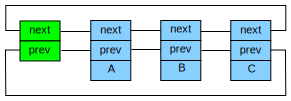
\includegraphics{defer/Linux_list}}
\caption{Linux Circular Linked List (\tco{list})}
\label{fig:defer:Linux Circular Linked List (list)}
\end{figure}

\begin{figure}[tb]
\centering
\resizebox{3in}{!}{
\includegraphics{defer/Linux_list_abbr}}
\caption{Linux Linked List Abbreviated}
\label{fig:defer:Linux Linked List Abbreviated}
\end{figure}

Although \co{rcu_assign_pointer()} and
\co{rcu_dereference()} can in theory be used to construct any
conceivable RCU-protected data structure, in practice it is often better
to use higher-level constructs.
Therefore, the \co{rcu_assign_pointer()} and
\co{rcu_dereference()}
primitives have been embedded in special RCU variants of Linux's
list-manipulation API.
Linux has four variants of doubly linked list, the circular
\co{struct list_head} and the linear
\co{struct hlist_head}/\co{struct hlist_node},
\co{struct hlist_nulls_head}/\co{struct hlist_nulls_node}, and
\co{struct hlist_bl_head}/\co{struct hlist_bl_node}
pairs.
The former is laid out as shown in
Figure~\ref{fig:defer:Linux Circular Linked List (list)},
where the green (leftmost) boxes represent the list header and the blue
(rightmost three) boxes represent the elements in the list.
This notation is cumbersome, and will therefore be abbreviated as shown in
Figure~\ref{fig:defer:Linux Linked List Abbreviated},
which shows only the non-header (blue) elements.

\begin{figure}[tb]
\centering
\resizebox{3in}{!}{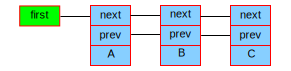
\includegraphics{defer/Linux_hlist}}
\caption{Linux Linear Linked List (\tco{hlist})}
\label{fig:defer:Linux Linear Linked List (hlist)}
\end{figure}

Linux's \co{hlist}\footnote{
	The ``h'' stands for hashtable, in which it reduces memory
	use by half compared to Linux's double-pointer circular
	linked list.}
is a linear list, which means that
it needs only one pointer for the header rather than the two
required for the circular list, as shown in
Figure~\ref{fig:defer:Linux Linear Linked List (hlist)}.
Thus, use of \co{hlist} can halve the memory consumption for the hash-bucket
arrays of large hash tables.
As before, this notation is cumbersome, so \co{hlist} structures will
be abbreviated in the same way \co{list_head}-style lists are, as shown in
Figure~\ref{fig:defer:Linux Linked List Abbreviated}.

A variant of Linux's \co{hlist}, named \co{hlist_nulls}, provides multiple
distinct \co{NULL} pointers, but otherwise uses the same layout as shown in
Figure~\ref{fig:defer:Linux Linear Linked List (hlist)}.
In this variant, a \co{->next} pointer having a zero low-order bit is
considered to be a pointer.
However, if the low-order bit is set to one, the upper bits identify
the type of \co{NULL} pointer.
This type of list is used to allow lockless readers to detect when a
node has been moved from one list to another.
For example, each bucket of a hash table might use its index to mark
its \co{NULL} pointer.
Should a reader encounter a \co{NULL} pointer not matching the index of
the bucket it started from, that reader knows that an element it was
traversing was moved to some other bucket during the traversal, taking
that reader with it.
The reader can use the \co{is_a_nulls()} function (which returns true
if passed an \co{hlist_nulls} \co{NULL} pointer) to determine when
it reaches the end of a list, and the \co{get_nulls_value()} function
(which returns its argument's \co{NULL}-pointer identifier) to fetch
the type of \co{NULL} pointer.
When \co{get_nulls_values()} returns an unexpected value, the reader
can take corrective action, for example, restarting its traversal from
the beginning.

\QuickQuiz{
	But what if an \co{hlist_nulls} reader gets moved to some other
	bucket and then back again?
}\QuickQuizAnswer{
	One way to handle this is to always move nodes to the beginning
	of the destination bucket, ensuring that when the reader reaches
	the end of the list having a matching \co{NULL} pointer, it will
	have searched the entire list.

	Of course, if there are too many move operations in a hash table
	with many elements per bucket, the reader might never reach the
	end of a list.
	One way of avoiding this in the common case is to keep hash
	tables well-tuned, thus with short lists.
	One way of detecting the problem and handling it is for the
	reader to terminate the search after traversing some large
	number of nodes, acquire the update-side lock, and redo the
	search, but this might introduce deadlocks.
	Another way of avoiding the problem entirely is for readers to
	search within RCU read-side critical sections, and to wait for
	an RCU grace period between successive updates.
	An intermediate position might wait for an RCU grace period
	every $N$ updates, for some suitable value of $N$.
}\QuickQuizEnd

More information on \co{hlist_nulls} is available in the Linux-kernel
source tree, with helpful example code provided in the
\path{rculist_nulls.rst} file (\path{rculist_nulls.txt} in older kernels).

Another variant of Linux's \co{hlist} incorporates bit-locking,
and is named \co{hlist_bl}.
This variant uses the same layout as shown in
Figure~\ref{fig:defer:Linux Linear Linked List (hlist)},
but reserves the low-order bit of the head pointer (``first'' in the
figure) to lock the list.
This approach also reduces memory usage, as it allows what would otherwise
be a separate spinlock to be stored with the pointer itself.

\begin{sidewaystable*}[htbp]
\rowcolors{1}{}{lightgray}
\renewcommand*{\arraystretch}{1.3}
\centering
\caption{RCU-Protected List APIs}
\label{tab:defer:RCU-Protected List APIs}
\footnotesize
\newlength{\cwa}\newlength{\cwb}\newlength{\cwc}\newlength{\cwd}
\IfNimbusAvail{
  \renewcommand{\ttdefault}{NimbusMonoN}
  \setlength{\cwa}{1.9in}\setlength{\cwb}{2.1in}
  \setlength{\cwc}{1.8in}\setlength{\cwd}{1.6in}
}{
  \setlength{\cwa}{1.95in}\setlength{\cwb}{2.15in}
  \setlength{\cwc}{1.9in}\setlength{\cwd}{1.7in}
}
\begin{tabular}{>{\raggedright\arraybackslash}p{\cwa}
    >{\raggedright\arraybackslash}p{\cwb}
    >{\raggedright\arraybackslash}p{\cwc}
    >{\raggedright\arraybackslash}p{\cwd}}
\toprule
\pmb{\tco{list}}: Circular doubly linked list &
    \pmb{\tco{hlist}}: Linear doubly linked list &
	\pmb{\tco{hlist_nulls}}: Linear doubly linked list with marked
	NULL pointer, with up to 31~bits of marking &
	    \pmb{\tco{hlist_bl}}: Linear doubly linked list with bit locking \\
\midrule
\multicolumn{4}{l}{{\bf Structures}} \\
\tco{struct list_head} &
    \tco{struct}{\tt ~}\tco{hlist_head} ~~~~~~~~~~~~~~
    \tco{struct}{\tt ~}\tco{hlist_node} &
	\tco{struct}{\tt ~}\tco{hlist_nulls_head}
	\tco{struct}{\tt ~}\tco{hlist_nulls_node} &
	    \tco{struct}{\tt ~}\tco{hlist_bl_head}
	    \tco{struct}{\tt ~}\tco{hlist_bl_node} \\
\multicolumn{4}{l}{{\bf Initialization}} \\
&
    \tco{INIT_LIST_HEAD_RCU()} &
	&
	    \\
\multicolumn{4}{l}{{\bf Full traversal}} \\
\tco{list_for_each_entry_rcu()}
\tco{list_for_each_entry_lockless()} &
    \tco{hlist_for_each_entry_rcu()}
    \tco{hlist_for_each_entry_rcu_bh()}
    \tco{hlist_for_each_entry_rcu_notrace()} &
	\tco{hlist_nulls_for_each_entry_rcu()}
	\tco{hlist_nulls_for_each_entry_safe()} &
	    \tco{hlist_bl_for_each_entry_rcu()} \\
\multicolumn{4}{l}{{\bf Resume traversal}} \\
\tco{list_for_each_entry_continue_rcu()}
\tco{list_for_each_entry_from_rcu()} &
    \tco{hlist_for_each_entry_continue_rcu()}
    \tco{hlist_for_each_entry_continue_rcu_bh()}
    \tco{hlist_for_each_entry_from_rcu()} &
	&
	    \\
\multicolumn{4}{l}{{\bf Stepwise traversal}} \\
\tco{list_entry_rcu()}
\tco{list_entry_lockless()}
\tco{list_first_or_null_rcu()}
\tco{list_next_rcu()}
\tco{list_next_or_null_rcu()} &
    \multicolumn{1}{p{1.2in}}{\tco{hlist_first_rcu()}
			      \tco{hlist_next_rcu()}
			      \tco{hlist_pprev_rcu()}} &
	\tco{hlist_nulls_first_rcu()}
	\tco{hlist_nulls_next_rcu()} &
	    \tco{hlist_bl_first_rcu()} \\
\multicolumn{4}{l}{{\bf Add}} \\
\multicolumn{1}{p{1.2in}}{\tco{list_add_rcu()}
			  \tco{list_add_tail_rcu()}} &
    \tco{hlist_add_before_rcu()}
    \tco{hlist_add_behind_rcu()}
    \tco{hlist_add_head_rcu()}
    \tco{hlist_add_tail_rcu()} &
	\tco{hlist_nulls_add_head_rcu()} &
	    \tco{hlist_bl_add_head_rcu()}
	    \tco{hlist_bl_set_first_rcu()} \\
\multicolumn{4}{l}{{\bf Delete}} \\
\tco{list_del_rcu()} &
    \multicolumn{1}{p{1.2in}}{\tco{hlist_del_rcu()}
			      \tco{hlist_del_init_rcu()}} &
	\tco{hlist_nulls_del_rcu()}
	\tco{hlist_nulls_del_init_rcu()} &
	    \tco{hlist_bl_del_rcu()}
	    \tco{hlist_bl_del_init_rcu()} \\
\multicolumn{4}{l}{{\bf Replace}} \\
\tco{list_replace_rcu()} &
    \tco{hlist_replace_rcu()} &
	&
	    \\
\multicolumn{4}{l}{{\bf Splice}} \\
\tco{list_splice_init_rcu()} &
    \tco{list_splice_tail_init_rcu()} &
	&
	    \\
\bottomrule
\end{tabular}
\end{sidewaystable*}

The API members for these linked-list variants are summarized in
Table~\ref{tab:defer:RCU-Protected List APIs}.
More information is available in the \path{Documentation/RCU}
directory of the Linux-kernel source tree and at
Linux Weekly News~\cite{PaulEMcKenney2019RCUAPI}.

However, the remainder of this section expands on the use of
\co{list_replace_rcu()}, given that this API member gave RCU its name.
This API member is used to carry out more complex updates in which an
element in the middle of the list having multiple fields is atomically
updated, so that a given reader sees either the old set of values or
the new set of values, but not a mixture of the two sets.
For example, each node of a linked list might have integer fields
\co{->a}, \co{->b}, and \co{->c}, and it might be necessary to update
a given node's fields from 5, 6, and 7 to 5, 2, and 3, respectively.

The code implementing this atomic update is straightforward:

\begin{fcvlabel}[ln:defer:Canonical RCU Replacement Example (2nd)]
\begin{VerbatimN}[samepage=true,commandchars=\\\[\],firstnumber=15]
q = kmalloc(sizeof(*p), GFP_KERNEL);	\lnlbl[kmalloc]
*q = *p;				\lnlbl[copy]
q->b = 2;				\lnlbl[update1]
q->c = 3;				\lnlbl[update2]
list_replace_rcu(&p->list, &q->list);	\lnlbl[replace]
synchronize_rcu();			\lnlbl[sync_rcu]
kfree(p);				\lnlbl[kfree]
\end{VerbatimN}
\end{fcvlabel}

\begin{figure}[tbp]
\centering
\resizebox{2.7in}{!}{\includegraphics{defer/RCUReplacement}}
\caption{RCU Replacement in Linked List}
\label{fig:defer:RCU Replacement in Linked List}
\end{figure}

The following discussion walks through this code, using
Figure~\ref{fig:defer:RCU Replacement in Linked List} to illustrate
the state changes.
The triples in each element represent the values of fields \co{->a},
\co{->b}, and \co{->c}, respectively.
The red-shaded elements might be referenced by readers,
and because readers do not synchronize directly with updaters,
readers might run concurrently with this entire replacement process.
Please note that backwards pointers and the link from the tail to the
head are omitted for clarity.

The initial state of the list, including the pointer \co{p},
is the same as for the deletion example, as shown on the
first row of the figure.

The following text describes how to replace the \co{5,6,7} element
with \co{5,2,3} in such a way that any given reader sees one of these
two values.

\begin{fcvref}[ln:defer:Canonical RCU Replacement Example (2nd)]
Line~\lnref{kmalloc} allocates a replacement element,
resulting in the state as shown in the second row of
Figure~\ref{fig:defer:RCU Replacement in Linked List}.
At this point, no reader can hold a reference to the newly allocated
element (as indicated by its green shading), and it is uninitialized
(as indicated by the question marks).

Line~\lnref{copy} copies the old element to the new one, resulting in the
state as shown in the third row of
Figure~\ref{fig:defer:RCU Replacement in Linked List}.
The newly allocated element still cannot be referenced by readers, but
it is now initialized.

Line~\lnref{update1} updates \co{q->b} to the value ``2'', and
line~\lnref{update2} updates \co{q->c} to the value ``3'',
as shown on the fourth row of
Figure~\ref{fig:defer:RCU Replacement in Linked List}.
Note that the newly allocated structure is still inaccessible to readers.

Now, line~\lnref{replace} does the replacement, so that the new element is
finally visible to readers, and hence is shaded red, as shown on
the fifth row of
Figure~\ref{fig:defer:RCU Replacement in Linked List}.
At this point, as shown below, we have two versions of the list.
Pre-existing readers might see the \co{5,6,7} element (which is
therefore now shaded yellow), but
new readers will instead see the \co{5,2,3} element.
But any given reader is guaranteed to see one set of values or the
other, not a mixture of the two.

After the \co{synchronize_rcu()} on line~\lnref{sync_rcu} returns,
a grace period will have elapsed, and so all reads that started before the
\co{list_replace_rcu()} will have completed.
In particular, any readers that might have been holding references
to the \co{5,6,7} element are guaranteed to have exited
their RCU read-side critical sections, and are thus prohibited from
continuing to hold a reference.
Therefore, there can no longer be any readers holding references
to the old element, as indicated its green shading in the sixth row of
Figure~\ref{fig:defer:RCU Replacement in Linked List}.
As far as the readers are concerned, we are back to having a single version
of the list, but with the new element in place of the old.

After the \co{kfree()} on line~\lnref{kfree} completes, the list will
appear as shown on the final row of
Figure~\ref{fig:defer:RCU Replacement in Linked List}.
\end{fcvref}

Despite the fact that RCU was named after the replacement case,
the vast majority of RCU usage within the Linux kernel relies on
the simple independent insertion and deletion, as was shown in
Figure~\ref{fig:defer:Multiple RCU Data-Structure Versions} in
Section~\ref{sec:defer:Maintain Multiple Versions of Recently Updated Objects}.

The next section looks at APIs that assist developers in debugging
their code that makes use of RCU.

\subsubsection{RCU Has Diagnostic APIs}
\label{sec:defer:RCU Has Diagnostic APIs}

\begin{table}[tb]
\renewcommand*{\arraystretch}{1.15}
\footnotesize
\centering
\begin{tabular}{ll}
\toprule
Category &
	Primitives \\
\midrule
Mark RCU pointer &
	\tco{__rcu} \\
\midrule
Debug-object support &
	\tco{init_rcu_head()} \\
&	\tco{destroy_rcu_head()} \\
&	\tco{init_rcu_head_on_stack()} \\
&	\tco{destroy_rcu_head_on_stack()} \\
\midrule
Stall-warning control &
	\tco{rcu_cpu_stall_reset()} \\
\midrule
Callback checking &
	\tco{rcu_head_init()} \\
&	\tco{rcu_head_after_call_rcu()} \\
\midrule
lockdep support &
	\tco{rcu_read_lock_held()} \\
&	\tco{rcu_read_lock_bh_held()} \\
&	\tco{rcu_read_lock_sched_held()} \\
&	\tco{srcu_read_lock_held()} \\
&	\tco{rcu_is_watching()} \\
&	\tco{RCU_LOCKDEP_WARN()} \\
&	\tco{RCU_NONIDLE()} \\
&	\tco{rcu_sleep_check()} \\
\bottomrule
\end{tabular}
\caption{RCU Diagnostic APIs}
\label{tab:defer:RCU Diagnostic APIs}
\end{table}

Table~\ref{tab:defer:RCU Diagnostic APIs}
shows RCU's diagnostic APIs.

The \co{__rcu} marks an RCU-protected pointer, for example,
\qtco{struct foo __rcu *p;}.
Pointers that might be passed to \co{rcu_dereference()} can be marked,
but pointers holding values returned from \co{rcu_dereference()}
should not be.
Providing these markings on variables, structure fields, function
parameters, and return values allow the Linux kernel's \co{sparse}
tool to detect situtations where RCU-protected pointers are
incorrectly accessed using plain C-language loads and stores.

Debug-object support is automatic for any \co{rcu_head} structures
that are part of a structure obtained from the Linux kernel's
memory allocators, but those building their own special-purpose
memory allocators can use \co{init_rcu_head()} and \co{destroy_rcu_head()}
at allocation and free time, respectively.
Those using \co{rcu_head} structures allocated on the function-call
stack (it happens!) may use \co{init_rcu_head_on_stack()}
before first use and \co{destroy_rcu_head_on_stack()} after last use,
but before returning from the function.
Debug-object support allows detection of bugs involving passing the
same \co{rcu_head} structure to \co{call_rcu()} and friends in
quick succession, which is the \co{call_rcu()} counterpart to the
infamous double-free class of memory-allocation bugs.

Stall-warning control is provided by \co{rcu_cpu_stall_reset()}, which
allows the caller to suppress RCU CPU stall warnings for the remainder
of the current grace period.
RCU CPU stall warnings help pinpoint situations where an RCU read-side
critical section runs for an excessive length of time, and it is useful
for things like kernel debuggers to be able to suppress them, for example,
when encountering a breakpoint.

Callback checking is provided by \co{rcu_head_init()} and
\co{rcu_head_after_call_rcu()}.
The former is invoked on an \co{rcu_head} structure before it is passed
to \co{call_rcu()}, and then \co{rcu_head_after_call_rcu()} will
check to see if the callback is has been invoked with the specified
function.

Support for lockdep~\cite{JonathanCorbet2006lockdep} includes
\co{rcu_read_lock_held()},
\co{rcu_read_lock_bh_held()},
\co{rcu_read_lock_sched_held()}, and
\co{srcu_read_lock_held()},
each of which returns \co{true} if invoked within the corresponding
type of RCU read-side critical section.

\QuickQuiz{
	Why isn't there a \co{rcu_read_lock_tasks_held()} for Tasks RCU?
}\QuickQuizAnswer{
	Because Tasks RCU does not have read-side markers.
	Instead, Tasks RCU read-side critical sections are
	bounded by voluntary context switches.
}\QuickQuizEnd

Because \co{rcu_read_lock()} cannot be used from the idle loop,
and because energy-efficiency concerns have caused the idle loop
to become quite ornate, \co{rcu_is_watching()} returns true if
invoked in a context where use of \co{rcu_read_lock()} is legal.
Note again that \co{srcu_read_lock()} may be used from idle and
even offline CPUs, which means that \co{rcu_is_watching()} does not
apply to SRCU.

\co{RCU_LOCKDEP_WARN()} emits a warning if lockdep is enabled and if
its argument evaluated to \co{true}.
For example, \co{RCU_LOCKDEP_WARN(!rcu_read_lock_held())} would emit a
warning if invoked outside of an RCU read-side critical section.

\co{RCU_NONIDLE()} may be used to force RCU to watch when executing
the statement that is passed in as the sole argument.
For example, \co{RCU_NONIDLE(WARN_ON(!rcu_is_watching()))}
would never emit a warning.
However, changes in the 2020--2021 timeframe extend RCU's reach deeper
into the idle loop, which should greatly reduce or even eliminate the
need for \co{RCU_NONIDLE()}.

Finally,  \co{rcu_sleep_check()} emits a warning if invoked within
an RCU, RCU-bh, or RCU-sched read-side critical section.

\subsubsection{Where Can RCU's APIs Be Used?}
\label{sec:defer:Where Can RCU's APIs Be Used?}

\begin{figure}[tb]
\centering
\resizebox{3in}{!}{\includegraphics{defer/RCUenvAPI}}
\caption{RCU API Usage Constraints}
\label{fig:defer:RCU API Usage Constraints}
\end{figure}

Figure~\ref{fig:defer:RCU API Usage Constraints}
shows which APIs may be used in which in-kernel environments.
The RCU read-side primitives may be used in any environment, including NMI,
the RCU mutation and asynchronous grace-period primitives may be used in any
environment other than NMI, and, finally, the RCU synchronous grace-period
primitives may be used only in process context.
The RCU list-traversal primitives include \co{list_for_each_entry_rcu()},
\co{hlist_for_each_entry_rcu()}, etc.
Similarly, the RCU list-mutation primitives include
\co{list_add_rcu()}, \co{hlist_del_rcu()}, etc.

Note that primitives from other families of RCU may be substituted,
for example, \co{srcu_read_lock()} may be used in any context
in which \co{rcu_read_lock()} may be used.

\subsubsection{So, What \emph{is} RCU Really?}
\label{sec:defer:So, What is RCU Really?}

At its core, RCU is nothing more nor less than an API that supports
publication and subscription for insertions, waiting for all RCU readers
to complete, and maintenance of multiple versions.
That said, it is possible to build higher-level constructs
on top of RCU, including the reader-writer-locking, reference-counting,
and existence-guarantee constructs listed in
Section~\ref{sec:defer:RCU Usage}.
Furthermore, I have no doubt that the Linux community will continue to
find interesting new uses for RCU,
just as they do for any of a number of synchronization
primitives throughout the kernel.

Of course, a more-complete view of RCU would also include
all of the things you can do with these APIs.

However, for many people, a complete view of RCU must include sample
RCU implementations.
Appendix~\ref{chp:app:``Toy'' RCU Implementations} therefore presents a series
of ``toy'' RCU implementations of increasing complexity and capability,
though others might prefer the classic
``User-Level Implementations of Read-Copy
Update''~\cite{MathieuDesnoyers2012URCU}.
For everyone else, the next section gives an overview of some RCU use cases.
